\chapter{Experimentos y resultados}\label{chapter:Results}

En este capítulo se presentan los experimentos realizados para evaluar el desempeño de los modelos propuestos: \textit{\textbf{LinearAEC}} y \textit{\textbf{VAE}}.  Se enuncian las métricas empleadas para evaluarlos, así como también la herramienta utilizada para visualizar el espacio latente conformado por los vectores de codificación. Finalmente se muestran los resultados obtenidos en varios ejemplos y se ofrece un análisis a partir de los mismos.

%\section{Generación de los datos}
\section{Consideraciones de la etapa de experimentación}\label{4-Consideraciones}

La generación de un conjunto de soluciones para instancias del VRP con cantidad de clientes considerables, resulta computacionalmente costoso. A ello se le suman los altos requerimientos de cómputo que demanda el proceso de entrenamiento. Por estas razones, se diseñó un marco experimental que fuera factible de ejecutar con recursos limitados.

El equipo de cómputo donde se realizaron los experimentos posee las siguientes propiedades:

\begin{description}
	\item[Memoria:] 16GB - RAM
	\item[Procesador:] \textit{AMD A10-8700P Radeon R6}
	\item[Arquitectura:] \textit{64 bits} 
\end{description}

La implementación de la solución se desarrolló en el lenguaje de programación \textit{Python} y auxiliado del \textit{framework Keras} \cite{keras}. Este último es una biblioteca de código abierto implementada en \textit{Python} y diseñada para posibilitar la experimentación de técnicas de aprendizaje profundo mediante redes neuronales. Sus principales ventajas consisten en ser amigable para el usuario, modular y extensible, de ahí su selección.

Como parte de esta etapa de experimentación, se realizaron varios intentos progresivos de entrenamiento. Se comenzó por conjuntos de datos pequeños hasta finalmente probar con otros de mayor dimensión y así, observar el desempeño con el aumento de los datos. En cada experimento la cantidad de datos destinados para la evaluación del modelo representa el $20\%$ del total, el 80\% restante se conforma de los datos de entrenamiento.

El proceso de aprendizaje pertenece a la categoría de aprendizaje no supervisado debido a que el conjunto de datos está formado por pares de la forma $(M, M)$, donde $M$ constituyen a las matrices binarias de entrada que representan las soluciones del VRP, y a su vez, su respectiva etiqueta o predicción esperada. El objetivo principal evaluado fue la capacidad de generación de soluciones válidas a partir de los vectores de contexto. De esta forma se determina si los vectores codificados son capaces de respresentar de manera continua a las soluciones del problema de enrutamiento.

El entorno de experimentación se desplegó mediante un módulo nombrado \textbf{Evaluador}, que se encarga de iniciar y relacionar la ejecución de los pasos comprendidos en este proceso. El evaluador recibe como argumentos la configuración de los parámetros necesarios para el experimento, el modelo a evaluar (LinearAEC, VAE u otro que cumpla la misma estructura definida en \ref{3-GenStruct}), una función generadora de soluciones del VRP y las métricas empleadas.

Para evaluar los resultados de cada experimento se formularon varias métricas cuantitativas con el fin de comparar la reconstrucción de las soluciones de entrada obtenidas por el \textit{decoder}. Estas se aplican sobre los conjuntos de entrenamiento, validación y prueba que se forman inicialmente con el generador de soluciones. Una vez finalizado el proceso de aprendizaje del modelo particular, se establecen las métricas a partir de una solución de entrada $X$ y su reconstrucción $X_p$:

\subsubsection{Métricas de evaluación}
\begin{description}
	\item[solución válida (valid): ] su valor es 1 si la solución $X_p$ es válida, en otro caso será 0.
	
	\item[mse:] valor del error cuadrático medio entre $X$ y $X_p$.
	
	\item[cantidad de rutas (eqRoutesNumber): ] su valor es 1 si la solución $X_p$ posee la misma cantidad de rutas que la solución $X$, en otro caso será 0.
	
	\item[longitud de rutas (eqRoutesSize): ] su valor es 1 si el conjunto formado por las longitudes de cada ruta en la solución $X$ es igual al conjunto correspondiente para la solución $X_p$, en otro caso será 0.
	
	%\item[inicios de rutas (eqRoutesStarts): ] su valor es 1 si el conjunto formado por los clientes iniciales de cada ruta en la solución $X_p$ es igual al conjunto correspondiente para la solución $X_p$, en otro caso será 0.
	
	%\item[finales de rutas (eqRoutesFinals): ] su valor es 1 si el conjunto formado por los clientes finales de cada ruta en la solución $X_p$ es igual al conjunto correspondiente para la solución $X_p$, en otro caso será 0.
\end{description}

Como se aplican sobre los conjuntos de datos antes mencionados, se calcula el promedio de cada una de ellas en el conjunto completo. 

En la siguiente sección se precisa mejor en qué consiste el experimento general elaborado y se ejemplifica el comportamiento de los modelos implicados con varias configuraciones del experimento.

\subsection{Descripción del marco experimental}

El experimento parte de la creación de una instancia del módulo Evaluador a partir de los argumentos que recibe. La configuración inicial consiste en los siguientes parámetros:
\begin{description}
	\item[\textbf{$n$}:] cantidad de clientes 
	\item[\textbf{$r$}:] cantidad de rutas de las soluciones 
	\item[\textbf{$train$}:] tamaño del conjunto de entrenamiento
	\item[\textbf{$val$}: ] tamaño del conjunto de evaluación
	\item[\textbf{$test$}:] tamaño del conjunto de prueba
	\item[\textbf{$epochs$}:] cantidad de épocas del entrenamiento
\end{description}

También hay que seleccionar el modelo que se evaluará, en ese caso los posibles son las dos propuestas ofrecidas:  \textit{\textbf{LinearAEC}} y \textit{\textbf{VAE}}. Con cada instancia del evaluador se realizará el mismo experimento en ambos modelos para establecer comparaciones con respecto a su rendimiento y capacidad.

La visualización de los datos juega un papel crucial en las aplicaciones de aprendizaje automático, facilitando por lo general, la interpretación y clasificación de los mismos. Por esta razón, se graficó el espacio latente conformado por los vectores reales de codificación mediante una herramienta conocida como \textit{t-SNE}, del inglés \textit{t-distributed stochastic neighbor embedding}. Esta técnica crea una distribución de probabilidad a partir de la distribución gaussiana que define las relaciones entre los puntos en el espacio de alta dimensión, en este caso, el espacio formado por los vectores de contexto denotados por $z$. Además, es capaz de preservar la estructura local y global de los datos.

Con el propósito de evidenciar las consideraciones expuestas en \ref{4-Consideraciones} y la descripción de esta sección, se presentan a continuación una serie de experimentos realizados. Para algunos de ellos, se muestran las funciones de pérdida sobre los datos de entrenamiento y validación, los valores de las métricas definidas y el espacio formado por los puntos de codificación.

\subsection{Ejemplos de experimentos realizados}

\subsubsection{Escenario 1}

La configuración incial del Evaluador se muestra en el cuadro \ref{case1}. Para este escenario el conjunto de datos lo forman soluciones de 25 clientes y 7 rutas 

\begin{table}[h]
	\centering
	\caption{Configuración del experimento en el escenario 1}
	\begin{tabular}{|c|c|c|c|c|c|}
		\hline
		\textbf{n} & \textbf{r} & \textbf{train} & \textbf{val} & \textbf{test} & \textbf{epochs} \\
		\hline
		25 & 7 & 5000 & 1000 & 1000 & 10 \\
		\hline
	\end{tabular}
	\label{case1}
\end{table}

Luego de aplicar las métricas en los conjuntos de entrenamiento, validación y prueba de ambos modelos, se obtienen los resultados resumidos en los cuadros \ref{case1AEC} y \ref{case1VAE}:

\begin{table}[!h]
	\centering
	\caption{Resultado de las métricas en el escenario 1 para el modelo LinearAEC}
	\begin{tabular}{|c|c|c|c|c|}
		\hline
		\textbf{conjunto} & \textbf{ valid} & \textbf{mse} & \textbf{eqRoutesNumber} & \textbf{eqRoutesSize}  \\
		\hline
		\textit{train} & 0.8873 & 0.0264 & 0.0007 & 0.0006 \\
		\hline
		\textit{val} & 0.893 & 0.0268 & 0.002 & 0.0015 \\
		\hline
		\textit{test} & 0.8885 & 0.0268 & 0.0005 & 0.0005 \\
		\hline
		
	\end{tabular}
	\label{case1AEC}
\end{table}

\begin{table}[!h]
	\centering
	\caption{Resultado de las métricas en el escenario 1 para el modelo VAE}
	\begin{tabular}{|c|c|c|c|c|}
		\hline
		\textbf{conjunto} & \textbf{ valid} & \textbf{mse} & \textbf{eqRoutesNumber} & \textbf{eqRoutesSize}  \\
		\hline
		\textit{train} & 0.8803 & 0.0274 & 0.0023 & 0.0021 \\
		\hline
		\textit{val} & 0.87 & 0.0278 & 0.002 & 0.0015 \\
		\hline
		\textit{test} & 0.8765 & 0.0278 & 0.0035 & 0.0025 \\
		\hline
		
	\end{tabular}
	\label{case1VAE}
\end{table}

Los gráficos en \ref{loss_case1} muestran el comportamiento de las funciones de pérdida durante el entrenamiento de ambos modelos.

\begin{figure}[!h]
	\label{loss_case1}
	\subfigure[Pérdida en el modelo LinearAECs]{ 
		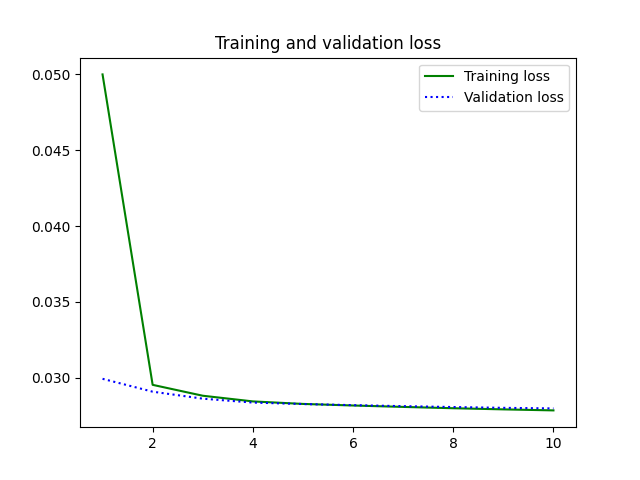
\includegraphics[width=2.9in]{Graphics/experiments/lossFunctions/loss_case1_AEC.png}	
 	}
	\subfigure[Pérdida en el modelo VAE]{ 
		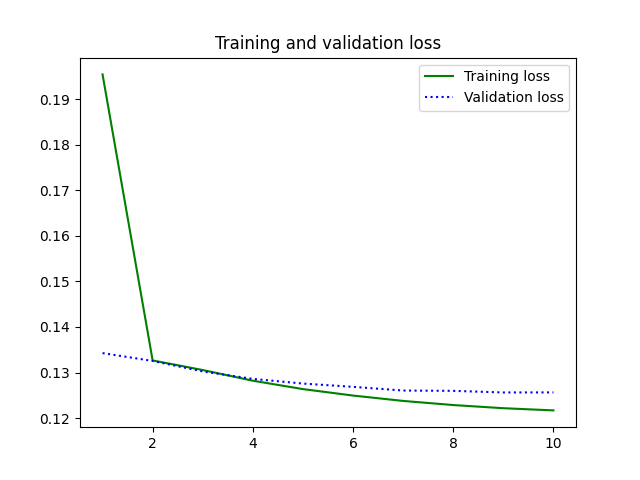
\includegraphics[width=2.9in]{Graphics/experiments/lossFunctions/loss_case1_VAE.png}	
	}
\end{figure}



\begin{figure}[!h]
	\label{space_case1}
	\subfigure[Espacio latente en el conjunto de entrenamiento del modelo LinearAEC]{ 
		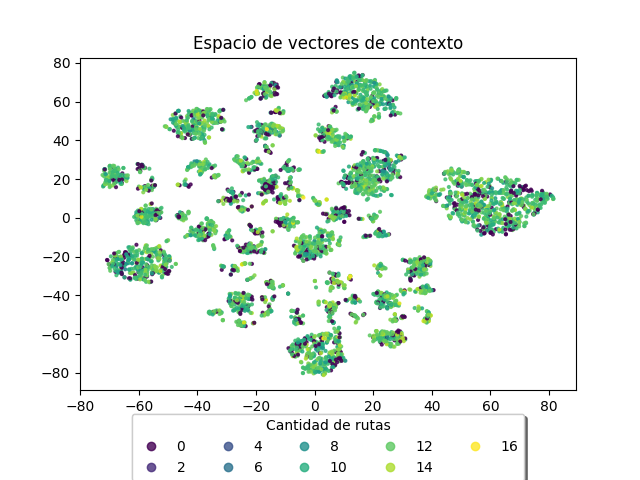
\includegraphics[scale=0.45]{Graphics/experiments/latentSpace/case1_data_AEC.png}	
	}
	\subfigure[Espacio latente en el conjunto de validación del modelo LinearAEC]{ 
		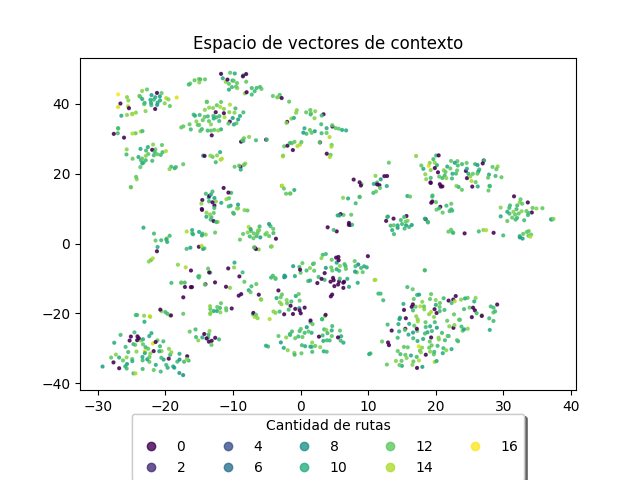
\includegraphics[scale=0.45]{Graphics/experiments/latentSpace/case1_val_AEC.png}	
	}
	%\subfigure[Espacio latente en el conjunto de prueba]{ 
	%	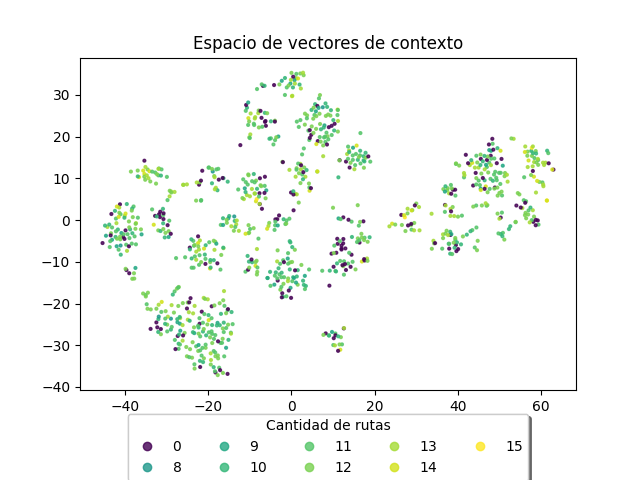
\includegraphics[scale=0.29]{Graphics/experiments/latentSpace/case1_test_AEC.png}	
	%}
\end{figure}

\begin{figure}[!h]
	\label{space_case1vae}
	\subfigure[Espacio latente en el conjunto de entrenamiento del modelo VAE]{ 
		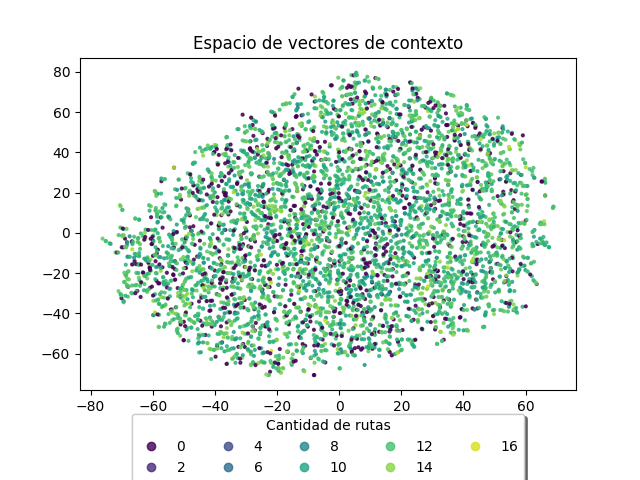
\includegraphics[scale=0.45]{Graphics/experiments/latentSpace/case1_data_VAE.png}	
	}
	\subfigure[Espacio latente en el conjunto de validación del modelo VAE]{ 
		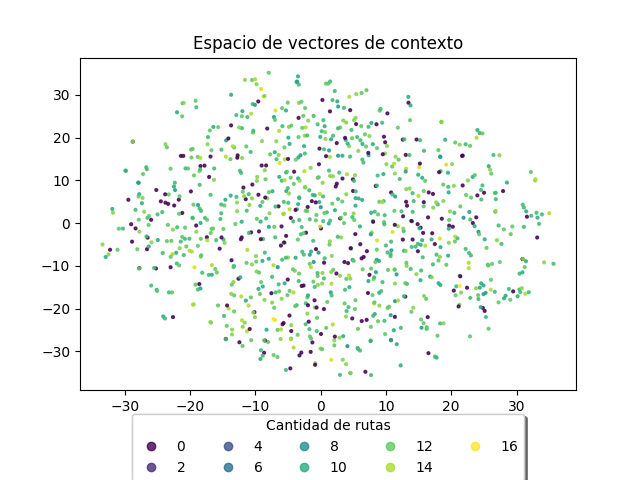
\includegraphics[scale=0.45]{Graphics/experiments/latentSpace/case1_val_VAE.png}	
	}
	%\subfigure[Espacio latente en el conjunto de prueba]{ 
	%	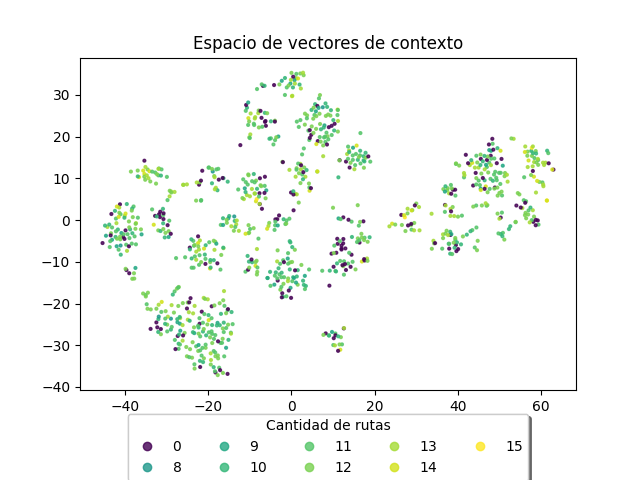
\includegraphics[scale=0.29]{Graphics/experiments/latentSpace/case1_test_AEC.png}	
	%}
\end{figure}

\newpage

\subsubsection{Escenario 2}

La configuración incial del Evaluador se muestra en el cuadro \ref{case2}. Para este escenario el conjunto de datos lo forman soluciones de 20 clientes y 5 rutas 

\begin{table}[h]
	\centering
	\caption{Configuración del experimento en el escenario 2}
	\begin{tabular}{|c|c|c|c|c|c|}
		\hline
		\textbf{n} & \textbf{r} & \textbf{train} & \textbf{val} & \textbf{test} & \textbf{epochs} \\
		\hline
		20 & 5 & 10000 & 2000 & 2000 & 20 \\
		\hline
	\end{tabular}
	\label{case2}
\end{table}

Luego de aplicar las métricas en los conjuntos de entrenamiento, validación y prueba de ambos modelos, se obtienen los resultados resumidos en los cuadros \ref{case2AEC} y \ref{case2VAE}:

\begin{table}[!h]
	\centering
	\caption{Resultado de las métricas en el escenario 2 para el modelo LinearAEC}
	\begin{tabular}{|c|c|c|c|c|}
		\hline
		\textbf{conjunto} & \textbf{ valid} & \textbf{mse} & \textbf{eqRoutesNumber} & \textbf{eqRoutesSize}  \\
		\hline
		\textit{train} & 0.8982 & 0.0342 & 0.0013 & 0.0007 \\
		\hline
		\textit{val} & 0.8745 & 0.0345 & 0.001 & 0.0005 \\
		\hline
		\textit{test} & 0.897 & 0.0346 & 0.0 & 0.0 \\
		\hline
		
	\end{tabular}
	\label{case2AEC}
\end{table}

\begin{table}[!h]
	\centering
	\caption{Resultado de las métricas en el escenario 2 para el modelo VAE}
	\begin{tabular}{|c|c|c|c|c|}
		\hline
		\textbf{conjunto} & \textbf{ valid} & \textbf{mse} & \textbf{eqRoutesNumber} & \textbf{eqRoutesSize}  \\
		\hline
		\textit{train} & 0.8665 & 0.0354 & 0.0319 & 0.0024 \\
		\hline
		\textit{val} & 0.852 & 0.0357 & 0.0245 & 0.002 \\
		\hline
		\textit{test} & 0.874 & 0.0357 & 0.032 & 0.0015 \\
		\hline
		
	\end{tabular}
	\label{case2VAE}
\end{table}

Los gráficos en \ref{loss_case2} muestran el comportamiento de las funciones de pérdida durante el entrenamiento de ambos modelos.

\begin{figure}[!h]
	\label{loss_case2}
	\subfigure[Pérdida en el modelo LinearAECs]{ 
		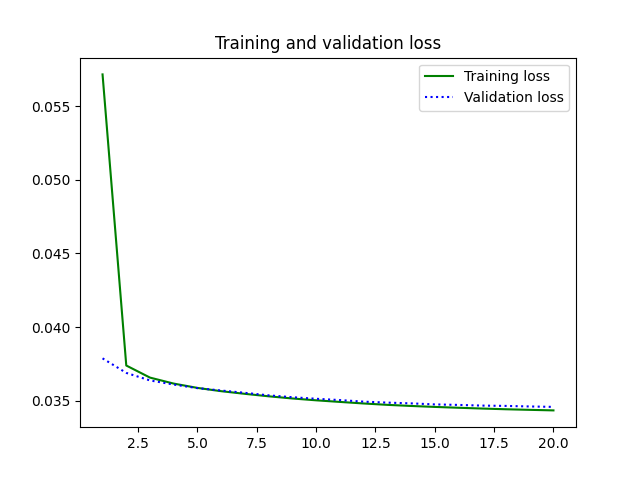
\includegraphics[width=2.9in]{Graphics/experiments/lossFunctions/loss_case2_AEC.png}	
	}
	\subfigure[Pérdida en el modelo VAE]{ 
		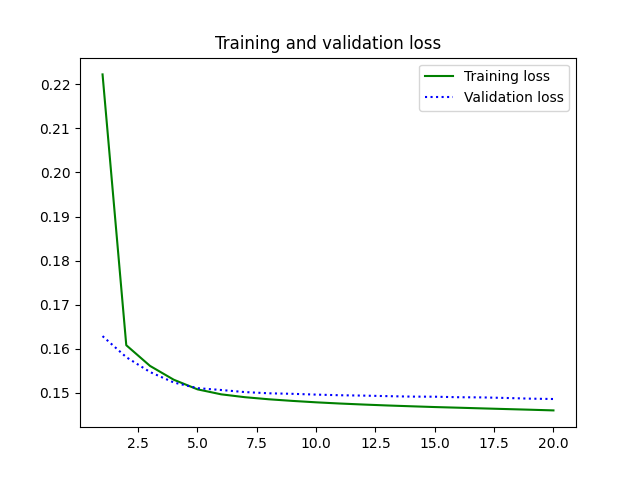
\includegraphics[width=2.9in]{Graphics/experiments/lossFunctions/loss_case2_VAE.png}	
	}
\end{figure}



\begin{figure}[!h]
	\label{space_case2}
	\subfigure[Espacio latente en el conjunto de entrenamiento del modelo LinearAEC]{ 
		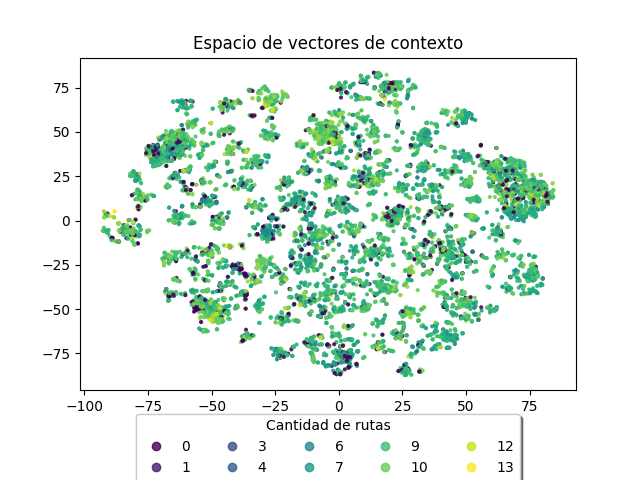
\includegraphics[scale=0.45]{Graphics/experiments/latentSpace/case2_data_AEC.png}	
	}
	\subfigure[Espacio latente en el conjunto de validación del modelo LinearAEC]{ 
		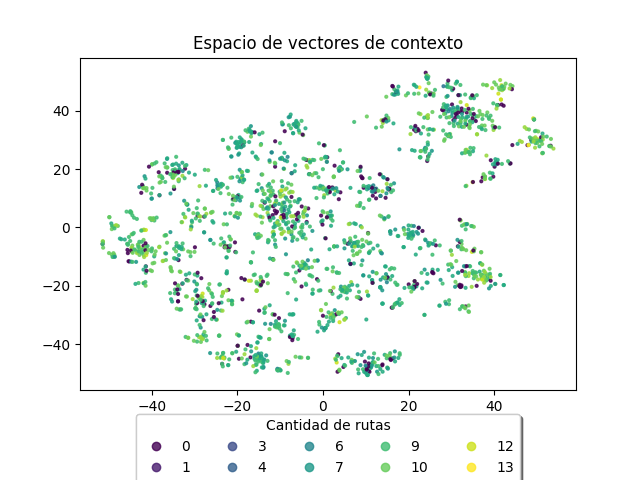
\includegraphics[scale=0.45]{Graphics/experiments/latentSpace/case2_val_AEC.png}	
	}
	%\subfigure[Espacio latente en el conjunto de prueba]{ 
	%	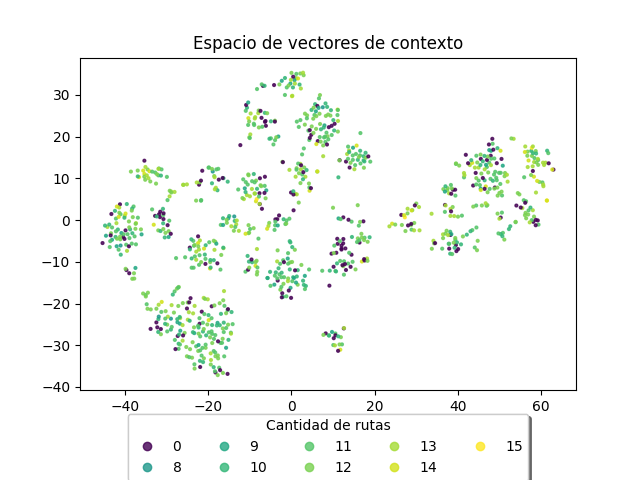
\includegraphics[scale=0.29]{Graphics/experiments/latentSpace/case1_test_AEC.png}	
	%}
\end{figure}

\begin{figure}[!h]
	\label{space_case2vae}
	\subfigure[Espacio latente en el conjunto de entrenamiento del modelo VAE]{ 
		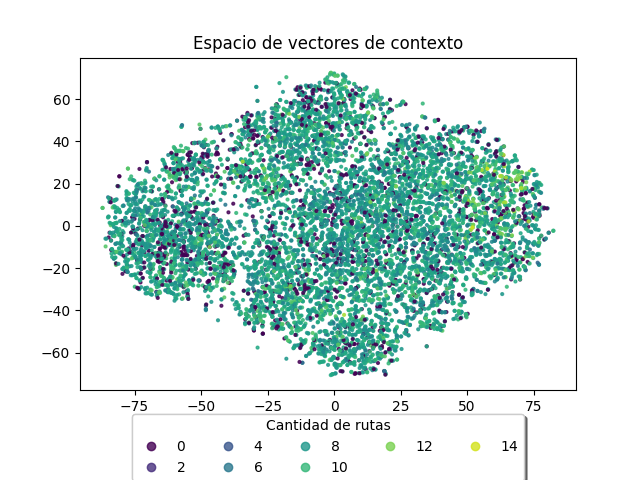
\includegraphics[scale=0.45]{Graphics/experiments/latentSpace/case2_data_VAE.png}	
	}
	\subfigure[Espacio latente en el conjunto de validación del modelo VAE]{ 
		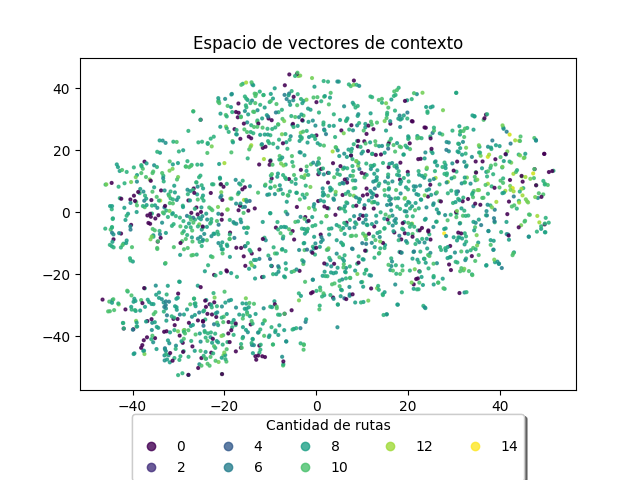
\includegraphics[scale=0.45]{Graphics/experiments/latentSpace/case2_val_VAE.png}	
	}
	%\subfigure[Espacio latente en el conjunto de prueba]{ 
	%	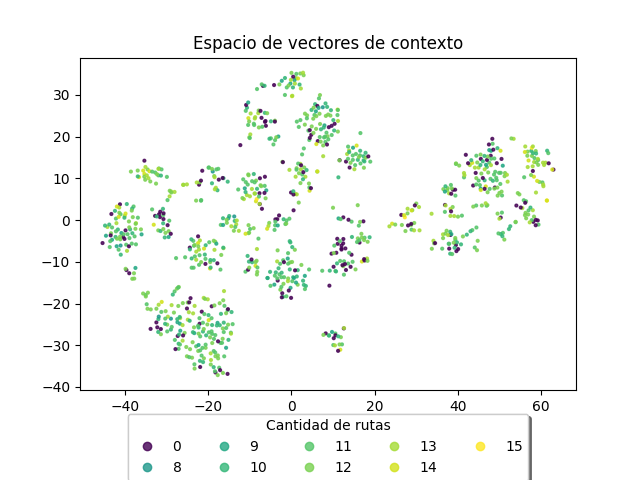
\includegraphics[scale=0.29]{Graphics/experiments/latentSpace/case1_test_AEC.png}	
	%}
\end{figure}

\newpage

\subsection{Análisis de resultados}

Luego de observar los resultados alcanzados en los escenarios anteriores se puede decir que el comportamiento de ambos modelos fue similar en todos los experimentos. Una de las causas es que poseen una arquitectura de capas y configuración de hiperparámetros semejante. 

En los gráficos de las funciones de pérdida se refleja el bajo error característico en los modelos \textit{autoencoders}, con un estilo similar a la pérdida resultante de los trabajos \cite{TrajectoryCompres, VAESparseData}. En el escenario 1, se observa cómo disminuye durante las dos primeras épocas y posteriormente se mantiene moderada.

Un valor de error pequeño no significa en este caso que la reconstrucción alcanzada en la salida se corresponda con la entrada. Este planteamieto se corrobora con los valores de las métricas \textit{eqRoutesNumber} y \textit{eqRoutesSize}, que evalúan la similitud entre una solución de entrada y su salida teniendo en cuenta la cantidad de rutas y las longitudes de cada ruta respectivamente. Pues como se observa en los cuadros \ref{case1AEC}, \ref{case1VAE}, \ref{case2AEC}, \ref{case2VAE}, sus valores son insignificantes y no aportan información sobre el parentezco de las soluciones con respecto a las características que examinan.

 %Debido a la estructura de las matrices $M$, que tienen una cantidad de posiciones igual a $n^2$ y en ellas a lo sumo habrán $n$ posiciones con valor distinto de cero ( $n$ rutas con un cliente distinto en cada una), la diferencia entre la matriz de entrada y la reconstruida a partir de la predicción es pequeña. A partir de esta interpretación, quizás resulte conveniente emplear otra representación vectorial de las soluciones durante el aprendizaje.
 
 A pesar de no alcanzar un nivel adecuado de reconstrucción, en todos los escenarios se comprueba un alto grado de generación de soluciones válidas para una cantidad fija de clientes. La métrica \textit{valid} confirma este efecto. Esta medida arroja en todos los escenarios, y para cada conjunto de datos (\textit{train}, \textit{valid}, \textit{test}), un porciento de generación mayor que $85\%$. Este rendimiento reafirma la capacidad de ambas propuestas como modelos generativos, haciendo posible la generación de nuevas soluciones al explorar el espacio continuo conformado.
 
 Este resultado constituye un logro para este trabajo debido a que se comprueba que las soluciones en el espacio discreto se pueden codificar a un vector real de menor dimensión y que estos, con alta probabilidad se decodifican a una posible solución válida. Se dice posible porque, en este trabajo, no se consideran las restricciones implícitas en el tipo de problema, solo interesa representar una solución a partir de un sistema de rutas.
  
 También se puede apreciar en la visualización de los espacios latentes conformados por las soluciones codificadas, una supremacía de puntos con cantidad de rutas cercana a la cantidad de rutas $r$ de los vectores con los que se entrenaron los modelos. Además, en un mismo modelo se observa que la distribución de puntos en el espacio latente posee una disposición similar. Por ejemplo, para el caso del modelo \textit{LinearAEC} los puntos se organizan formando pequeños conjuntos. A partir de esta interpretación, quizás resulte conveniente explorar ese espacio para descubrir otro tipo de relaciones. Como por ejemplo, determinar si esas agrupaciones están formadas por soluciones con características similares. 
 
 Durante esta etapa de experimentación se prepararon dos escenarios distintos para evaluar el desempeño de ambos modelos. Para ello se calcularon las métricas definidas y se visualizaron los espacios latentes correspondientes. Finalmente se concluye con la obtención de un alto grado de reconstrucción de soluciones válidas.
